% !TeX spellcheck = ru_RU_yo
%% -*- coding: utf-8 -*-
\documentclass[12pt,a4paper]{scrartcl} 
\usepackage[T1,T2A]{fontenc}
\usepackage[english,russian]{babel}
\usepackage[utf8]{inputenc}
\usepackage{geometry} 
\geometry{tmargin=2cm,bmargin=2cm,lmargin=3cm,rmargin=1.5cm}
\usepackage{indentfirst}
\usepackage{misccorr}
\usepackage{graphicx}
\usepackage{amsmath}
\usepackage{setspace}
\PassOptionsToPackage{hyphens}{url}
\usepackage[breaklinks]{hyperref}
\usepackage{minted}
\usepackage{textcomp}
\usepackage{comment}
\usepackage{soul}
\usepackage{array}
\usepackage{longtable}
\usepackage{multirow}
\usepackage{makecell}
\usepackage[stable]{footmisc}
\usepackage{listings}
\usepackage{tabularx,booktabs} 
\usepackage{fixme}
\fxsetup{status=draft}
\graphicspath{{images/}}
\usepackage{svg}
\svgpath{{images/}}

%Отключает нумерацию страницы
\pagestyle{empty}

%\titleformat*{\section}{\centering\bfseries}
%\titleformat*{\subsection}{\Large\bfseries}
%\titleformat*{\subsubsection}{\large\bfseries}
%\titleformat*{\paragraph}{\large\bfseries}
%\titleformat*{\subparagraph}{\large\bfseries}

% Команда для линии с нижним подчёркиванием, возможностью написания сверху текста на ней и текстом под ней.
\newcommand\superunderline[3]{$\underset{\text{#3}}{\text{\underline{\hspace{0.3cm}#1\hspace{#2}}}}$}

% Тоже самое, но ещё с отступом слева от текста (выравнивание по середине)
\newcommand\superunderlinec[3]{$\underset{\text{#3}}{\text{\underline{\hspace{#2}#1\hspace{#2}}}}$}

% "Прокаченные" типы колонок для LaTeX. Умеют выравнивать содержимое столбца по горизонтали и принимать фиксированный размер. Полезная вещь.
\newcolumntype{L}[1]{>{\raggedright\let\newline\\\arraybackslash\hspace{0pt}}m{#1}} % Выравнивание по левому краю.
\newcolumntype{C}[1]{>{\centering\let\newline\\\arraybackslash\hspace{0pt}}m{#1}} % Выравнивание по середине.
\newcolumntype{R}[1]{>{\raggedleft\let\newline\\\arraybackslash\hspace{0pt}}m{#1}} % Выравнивание по правому краю.

% Разработка 1993 года: команды, исправляющие неправильные отступы в шапке и подвале колонок в таблицах LaTeX. 
\newcommand\Tstrut{\rule{0pt}{2.6ex}}         % Введи \Tstrut если буквы в таблице налезли на верхнюю полоску
\newcommand\Bstrut{\rule[-0.9ex]{0pt}{0pt}}   % И \Bstrut если буквы "съехали" с середины колонки или наезжают на нижнюю полоску

%Настройки для того, чтобы была возможность переносить строки внутри таблиц. Подробнее здесь:  https://tex.stackexchange.com/questions/2441/how-to-add-a-forced-line-break-inside-a-table-cell
\renewcommand\theadalign{bc}
\renewcommand\theadfont{\normalfont}
\renewcommand\theadgape{\Gape[0pt]}
\renewcommand\cellgape{\Gape[0pt]}

% Убираем варнинг о том что long table представляет собой слишком большой vbox
\makeatletter
\def\LT@start{%
  \let\LT@start\endgraf
  \endgraf\penalty\z@\vskip\LTpre
  \dimen@\pagetotal
  \advance\dimen@ \ht\ifvoid\LT@firsthead\LT@head\else\LT@firsthead\fi
  \advance\dimen@ \dp\ifvoid\LT@firsthead\LT@head\else\LT@firsthead\fi
  \advance\dimen@ \ht\LT@foot
  \edef\restore@vbadness{\vbadness\the\vbadness\relax}% (added)
  \vbadness=\@M % (added)
  \dimen@ii\vfuzz
  \vfuzz\maxdimen
    \setbox\tw@\copy\z@
    \setbox\tw@\vsplit\tw@ to \ht\@arstrutbox
    \setbox\tw@\vbox{\unvbox\tw@}%
  \vfuzz\dimen@ii
  \restore@vbadness % (added)
  \advance\dimen@ \ht
        \ifdim\ht\@arstrutbox>\ht\tw@\@arstrutbox\else\tw@\fi
  \advance\dimen@\dp
        \ifdim\dp\@arstrutbox>\dp\tw@\@arstrutbox\else\tw@\fi
  \advance\dimen@ -\pagegoal
  \ifdim \dimen@>\z@\vfil\break\fi
      \global\@colroom\@colht
  \ifvoid\LT@foot\else
    \advance\vsize-\ht\LT@foot
    \global\advance\@colroom-\ht\LT@foot
    \dimen@\pagegoal\advance\dimen@-\ht\LT@foot\pagegoal\dimen@
    \maxdepth\z@
  \fi
  \ifvoid\LT@firsthead\copy\LT@head\else\box\LT@firsthead\fi\nobreak
  \output{\LT@output}%
}
\makeatother

%Используется для построения подчеркивающих линий
\newlength{\ML}

\setlength{\parskip}{0.5cm}

%\thispagestyle{empty}

\begin{document}
	\phantom{fake text for spacing}
	% ТИТУЛЬНАЯ ЧАСТЬ
	\begin{center}
		\textbf{Министерство науки и высшего образования Российской Федерации} \\
		\textbf{ФГАОУ ВО «Волгоградский государственный университет»} \\
		\textbf{Институт Математики и информационных технологий} \\
		\textbf{Кафедра компьютерных наук и экспериментальной математики} \\
		
		\vspace{0.6cm}
		
		\hfill\begin{minipage}{0.4\textwidth}
		\begin{flushright}
			\textbf{\textsc{УТВЕРЖДАЮ:}} \\
			Зав. кафедрой \textit{КНЭМ} \\
			Клячин В.А.\\
			«\underline{\hspace{0.7cm}}» \underline{\hspace{2.5cm}} 20\underline{\hspace{0.7cm}} г.
		\end{flushright}
		\end{minipage}
		
		\vspace{0.6cm}
		
		\textbf{
			ИНДИВИДУАЛЬНОЕ ЗАДАНИЕ на ПРОИЗВОДСТВЕННУЮ ПРАКТИКУ (ПРЕДДИПЛОМНАЯ)
			\vspace{0.2cm}
		}
		
		\vspace{0.3cm}
		\renewcommand{\arraystretch}{1.5} %!!!
		
		\begin{tabular}{R{3cm}cc}
			Студент & \superunderlinec{\thead{Курбанов Эльдар \\ Ровшанович}}{1.0cm}{(ФИО)} &  \superunderlinec{\thead{МОСм-201}}{1.9cm}{(группа)}
			\vspace{0.6cm} \\
			Руководитель практики от ВолГУ & \superunderlinec{\thead{\phantom{fake text for align}\\Клячин В.А.}}{1.1cm}{(ФИО)} & \superunderlinec{\thead{зав. кафедрой КНЭМ,\\профессор, д.ф.-м.н.}}{0.7cm}{(должность, ученое звание и степень)} \\
			Ответственный за организацию практики от кафедры
 & \superunderlinec{\thead{\phantom{fake text for align}\\Клячин В.А.}}{1.1cm}{(ФИО)} & \superunderlinec{\thead{зав. кафедрой КНЭМ,\\профессор, д.ф.-м.н.}}{0.7cm}{(должность, ученое звание и степень)} \\
			%ragedleft?????? seriously, it works as right align. WTF????
			\multirow{3}{3cm}{\raggedleft Место прохождения практики \phantom{AlignAlign}} & \multicolumn{2}{c}{\underline{\hspace{0.2cm}Лаборатория <<Математического и программного обеспечения\hspace{1cm}}} \\
			& \multicolumn{2}{l}{\superunderlinec{\hspace{0.2cm}ЭВМ>> кафедры КНЭМ ИМИТ ФГАОУ ВолГУ\hspace{3.7cm}}{0cm}{(наименование учреждения, структурного подразделения)}} \\
			Сроки прохождения практики & \multicolumn{2}{l}{с <<29>> апреля 2022 г. \hspace{3cm} по <<16>> мая 2022 г.}
		\end{tabular}
	\end{center}
	%КОНЕЦ ТИТУЛЬНОЙ ЧАСТИ
	
	\newpage
	
	\vspace{0.1cm}
	%1 раздел
	1. Содержание и задания практики:
		%\newpage
		\begin{longtable}{| L{0.7cm} | L{1.9cm}| L{5.3cm} | L{1cm} | L{2.1cm} | L{1.7cm} |}
			\hline % Требуется для рисования горизонтальной линии.
			\centering{№ п/п} &	\centering{Этапы практики} & \centering{Содержание работы и задания этапов} & \Tstrut \centering{Коли-чество часов} & \Tstrut \centering{Календар-ные сроки проведе-ния} & Форма отчётности \\
			\hline
			% Используем Bstrut и Tstrut в необходимых местах чтобы чинить вёрстку таблицы. Как можете заметить, выше пришлось вручную переносить слова при помощи "-". К сожалению, Bstrut и Tstrut ломают автоматические переносы цельных слов в LaTeX.
			1 & \Tstrut Подгото-витель-ный этап \Bstrut & Решение организационных вопросов: установочная конференция, знакомство с задачами и программой практики, требованиями к отчетной документации; знакомство с объектами и особенностями предстоящей деятельности; инструктаж по технике безопасности & 10 & 29.04.2022 & Собеседование \\
			\hline
			2 & Ориентировочный этап & Знакомство с базовой организацией практики, изучение и анализ/обзор нормативно-правовой документации; знакомство с методами работы; изучение/обзор литературы; знакомство с методами исследования. & 18 & 30.04.2022-04.05.2022 & Собеседование. Письменный отчет (часть). \Bstrut \\
			\hline
			3 & Основной этап & Подготовка научно-аналитического обзора по выбранной тематике на основе последних публикаций в российских и зарубежных журналах для анализа существующих решений по заданной предметной области.
Построение функциональной модели или диаграммы классов для описания поставленной задачи (Описание структурных элементов исследования, их связи, возможные форматы представляемых в системе данных. Анализ особенностей решаемой задачи.). Представление методов оценки качества проектного решения (например, результатов тестирования). & 60 & 05.05.2022-12.05.2022 & Письменный отчёт (часть). \\
			\hline
			4 & Заключи-тельный этап & Подготовка отчета о прохождении практики. Выступление с докладом-презентацией. & 20 & 13.05.2022-16.05.2022 & Письменный отчет (оформление). Представление/защита результатов практики. \\
			\hline
		\end{longtable}
	
		2. Планируемые результаты практики:\\
		\textit{студент должен знать}: основы в области математики, программирования и информационных технологий; методы построения научной работы, современные методы сбора и анализа полученного материала, способы аргументации; основы построения научных обзоров, публикаций, рефератов и библиографий по тематике проводимых исследований на русском и английском языках; особенности распоряжения правами на
результаты интеллектуальной деятельности; формы и методы правовой охраны результатов интеллектуальной деятельности; современными технологиями проектирования и производства программного продукта; направления развития: компьютеров с традиционной (нетрадиционной) архитектурой; современных систем программных средств, операционных систем, операционных и сетевых оболочек, сервисных программ; тенденции развития функций и архитектур проблемно-ориентированных программных систем и комплексов в профессиональной деятельности; концептуальные положения функционального, логического, объектно-ориентированного и визуального направлений программирования, методы, способы и средства разработки программ в рамках этих направлений; современные методы разработки и реализации алгоритмов математических моделей на базе языков и пакетов прикладных программ моделирования; основные стандарты, нормы и правила разработки технической документации программных продуктов и программных комплексов.


		\textit{студент должен уметь}: находить, формулировать и решать стандартные задачи в собственной научно-исследовательской деятельности в области программирования и информационных технологий; решать научные задачи в связи с поставленной целью и в соответствии с выбранной методикой; решать задачи, связанные с использованием
результатов интеллектуальной деятельности и средств индивидуализации для создания инновационной продукции и услуг, в том числе ориентированных на зарубежные рынки; использовать технологии проектирования при создании программных продуктов; программировать для компьютеров с различной современной архитектурой; программировать в рамках функционального, логического, объектно-ориентированного и визуального направлений; разрабатывать и реализовывать алгоритмы математических моделей на базе языков и пакетов прикладных программ моделирования; подготовить техническую документацию программных продуктов.


		\textit{студент должен владеть умениями}: научно-исследовательской деятельности в области
программирования и информационных технологий; выступлений и научной
аргументации и профессиональной деятельности; выполнять оценку преимуществ новой
технологии по сравнению с аналогами; применения технологий проектирования при создании программных продуктов; выбора архитектуры и комплексирования современных компьютеров, систем, комплексов и сетей системного администрирования; разработки программ в рамках функционального, логического, объектно-ориентированного и визуального направлений; разработки и реализации алгоритмов их на базе языков и пакетов прикладных программ моделирования; подготовки технической документации.

		\vspace{0.5cm}

		\hfill\begin{minipage}{0.7\textwidth}
			Студент \hspace{0.2cm} \superunderlinec{\phantom{Курбанов Э.Р.}}{0.3cm}{(подпись)} \hspace{1.01cm} \superunderlinec{\phantom{Курбанов Э.Р.}}{0.49cm}{(расшифровка подписи)} \\
			\vspace{0.2cm}
		\end{minipage}
		\hfill\begin{minipage}{\textwidth}
			Руководитель практики от ВолГУ \hspace{0.2cm} \superunderlinec{\phantom{Курбанов Э.Р.}}{0.3cm}{(подпись)} \hspace{1cm} \superunderlinec{Клячин В.А.}{0.6cm}{(расшифровка подписи)} \\
		\end{minipage}
	    \hfill\begin{minipage}{\textwidth}
	     \hspace{0.6cm}Ответственный за организацию\\\phantom{для выравни}практики от кафедры\hspace{0.25cm} \superunderlinec{\phantom{Курбанов Э.Р.}}{0.3cm}{(подпись)} \hspace{1cm} \superunderlinec{Клячин В.А.}{0.6cm}{(расшифровка подписи)} \\
	    \end{minipage}
	
	\newpage
	
	% ТИТУЛЬНАЯ ЧАСТЬ
	\begin{center}
		\textbf{Министерство науки и высшего образования Российской Федерации} \\
		\textbf{ФГАОУ ВО «Волгоградский государственный университет»} \\
		\textbf{Институт математики и информационных технологий} \\
		\textbf{Кафедра компьютерных наук и экспериментальной математики} \\
		
		\vspace{0.6cm}
		
		\hfill\begin{minipage}{0.4\textwidth}
		\begin{flushright}
			\textbf{\textsc{УТВЕРЖДАЮ:}} \\
			Зав. кафедрой \textit{КНЭМ} \\
			Клячин В.А.\\
			«\underline{\hspace{0.7cm}}» \underline{\hspace{2.5cm}} 20\underline{\hspace{0.7cm}} г.
		\end{flushright}
		\end{minipage}
		
		\vspace{0.6cm}
		
		\textbf{
			ОТЧЕТ\\О ПРОХОЖДЕНИИ ПРОИЗВОДСТВЕННОЙ ПРАКТИКИ\\(ПРЕДДИПЛОМНАЯ)
			\vspace{0.2cm}
		}
		
		\vspace{0.3cm}
		\renewcommand{\arraystretch}{1.5} %!!!
		
		\begin{tabular}{R{3cm}cc}
			Студент & \superunderlinec{\thead{\normalfont{Курбанов Эльдар} \\ \normalfont{Ровшанович}}}{1.0cm}{(ФИО)} &  \superunderlinec{\thead{\normalfont{МОСм-201}}}{1.9cm}{(группа)}
			\vspace{0.6cm} \\
			Руководитель практики от ВолГУ & \superunderlinec{\thead{\normalfont{\phantom{fake text for align}}\\\normalfont{Клячин В.А.}}}{1.1cm}{(ФИО)} & \superunderlinec{\thead{\normalfont{зав. кафедрой КНЭМ,}\\\normalfont{профессор., д.ф.-м.н.}}}{0.7cm}{(должность, ученое звание и степень)} \\
			Ответственный за организацию практики от кафедры
			& \superunderlinec{\thead{\normalfont{\phantom{fake text for align}}\\\normalfont{Клячин В.А.}}}{1.1cm}{(ФИО)} & \superunderlinec{\thead{\normalfont{зав. кафедрой КНЭМ,}\\\normalfont{профессор., д.ф.-м.н.}}}{0.7cm}{(должность, ученое звание и степень)} \\
			%ragedleft?????? seriously, it works as right align. WTF????
			\multirow{3}{3cm}{\raggedleft Место прохождения практики \phantom{AlignAlign}} & \multicolumn{2}{c}{\underline{\hspace{0.2cm}Лаборатория <<Математического и программного обеспечения\hspace{1cm}}} \\
			& \multicolumn{2}{l}{\superunderlinec{\hspace{0.2cm}ЭВМ>> кафедры КНЭМ ИМИТ ФГАОУ ВолГУ\hspace{3.7cm}}{0cm}{(наименование учреждения, структурного подразделения)}} \\
			
			Сроки прохождения практики & \multicolumn{2}{c}{с <<29>> апреля 2022 г. \hspace{2cm} по <<16>> мая 2022 г.}
		\end{tabular}
	\end{center}
	%КОНЕЦ ТИТУЛЬНОЙ ЧАСТИ
	
	\newpage
	
	\begin{center}
		\textbf{1. Ход выполнения практики}
	\end{center}

\renewcommand\theadalign{bl}

	\begin{longtable}{| C{0.6cm} | C{2cm}| C{2cm} | L{5.5cm} | C{2.58cm} |}
		\hline % Требуется для рисования горизонтальной линии.
		№ п/п &	Этап практики & Дата & \centering Описание выполненной работы & \Tstrut Отметки руководителя о выполнении \\
		\hline
		% Используем Bstrut и Tstrut в необходимых местах чтобы чинить вёрстку таблицы. Как можете заметить, выше пришлось вручную переносить слова при помощи "-". К сожалению, Bstrut и Tstrut ломают автоматические переносы цельных слов в LaTeX.
		1 & Подготовительный этап & 29.04.2022 \Bstrut & Решение организационных вопросов: установочная конференция, знакомство с задачами и программой практики, требованиями к отчетной документации; знакомство с объектами и особенностями предстоящей деятельности; инструктаж по технике безопасности & \\
		\hline
		2 & Ориентировочный этап & 30.04.2022-04.05.2022 \Bstrut & Знакомство с базовой организацией практики, изучение и анализ/обзор нормативно-правовой документации; знакомство с методами работы; изучение/обзор литературы; знакомство с методами исследования. & \\
		\hline
		\multirow{10}{0.6cm}{\centering 3} & \multirow{10}{2cm}{\centering Основной этап} & 05.05.2022 \Bstrut & \Tstrut Подготовка научно-аналитического обзора по выбранной тематике на основе последних публикаций в российских и зарубежных журналах для анализа существующих решений по заданной предметной области. & \\
		\cline{3-5}
		& & 06.05.2022-11.05.2022 \Bstrut & \Tstrut Построение функциональной модели или диаграммы классов для описания поставленной задачи (Описание структурных элементов исследования, их связи, возможные форматы представляемых в системе данных. Анализ особенностей решаемой задачи.). & \\
		\cline{3-5}
		& & 12.05.2022 \Bstrut & \Tstrut Представление методов оценки качества проектного решения (например, результатов тестирования). & \\
		\hline
		4 & Заключительный этап & 13.05.2022-16.05.2022 \Bstrut & \Tstrut Подготовка отчета о прохождении практики. Выступление с докладом-презентацией. & \\
		\hline
		
	\end{longtable}

\renewcommand\theadalign{bc}
	
	\vspace{0.5cm}
	\hfill\begin{minipage}{0.7\textwidth}
		Студент \hspace{0.2cm} \superunderlinec{\phantom{Курбанов Э.Р.}}{0.3cm}{(подпись)} \hspace{1cm} \superunderlinec{Курбанов Э.Р.}{0.3cm}{(расшифровка подписи)} \\
	\end{minipage}
	
	%КОНЕЦ ПЕРВОЙ СЕКЦИИ
	
	\newpage
		
		\begin{center}
			\textbf{ОТЗЫВ РУКОВОДИТЕЛЯ ОТ УНИВЕРСИТЕТА} \\
			\vspace{0.5cm}
			\noindent
			\underline{\hspace{15cm}} \\
			\vspace{0.3cm}\underline{\hspace{15cm}} \\
			\vspace{0.3cm}\underline{\hspace{15cm}} \\
			\vspace{0.3cm}\underline{\hspace{15cm}} \\
			\vspace{0.3cm}\underline{\hspace{15cm}} \\
			\vspace{0.3cm}\underline{\hspace{15cm}} \\
			\vspace{0.3cm}\underline{\hspace{15cm}} \\
			\vspace{0.3cm}\underline{\hspace{15cm}} \\
			\vspace{0.3cm}\underline{\hspace{15cm}} \\
			\vspace{0.3cm}\underline{\hspace{15cm}} \\
			\vspace{0.3cm}\underline{\hspace{15cm}} \\
			\vspace{0.3cm}\underline{\hspace{15cm}} \\
			\vspace{0.3cm}\underline{\hspace{15cm}} \\
			\vspace{0.3cm}\underline{\hspace{15cm}} \\
			\vspace{0.3cm}\underline{\hspace{15cm}} \\
			\vspace{0.3cm}\underline{\hspace{15cm}} \\
			\vspace{0.3cm}\underline{\hspace{15cm}} \\
			\vspace{0.3cm}\underline{\hspace{15cm}} \\
		\end{center}
		
		\renewcommand{\arraystretch}{2} %!!!
		\renewcommand\theadalign{br}
		
		\begin{tabular}{R{5cm}cc}
			Зачёт по практике принят с оценкой & \superunderlinec{}{2.22cm}{(по 5-балльной шкале)} &  \superunderlinec{}{2.22cm}{(по 100-бальной шкале)} \\
			Ответственный за организацию практики от \phantom{sdfsdfsdfsdsdf} кафедры «\underline{\hspace{0.7cm}}» \underline{\hspace{2.1cm}} 20\underline{\hspace{0.6cm}} г. & \superunderlinec{}{2.22cm}{(подпись)} & \Tstrut\superunderlinec{Клячин В.А.}{1cm}{(расшифровка подписи)} \\
			Руководитель практики \phantom{sdfsdfsdfsdsdf} от ВолГУ «\underline{\hspace{0.7cm}}» \underline{\hspace{2.1cm}} 20\underline{\hspace{0.6cm}} г. & \superunderlinec{}{2.22cm}{(подпись)} & \Tstrut\superunderlinec{Клячин В.А.}{1cm}{(расшифровка подписи)} \\
		\end{tabular}
		
	\newpage
	
	\begin{center}
		\textbf{Приложения\footnote{Приложения к отчету о прохождении практики: (приводится материалы, указанные в индивидуальном плане на практику в графе «Форма отчетности», например, научно-исследовательская работа, презентации, конспект занятия и т.д.).}}
	\end{center}
	
	\tableofcontents
		
	\newpage
	
		\section*{Введение}
			Темой выпускной квалификационной работы является <<Система управления и формирования поведенческой стратегии автономного мобильного робота на основе визуального анализа окружающего пространства>>. 
			
			Целью ВКР\footnote{Выпускная квалификационная работа} является создание автономной системы управления мобильным роботом, а также системы самостоятельно принимающей решения о движении данного робота на основе визуальных данных, собираемых с лазерного сканера LiDAR, а также видеокамеры, установленной на шасси робота.
			
			Задачей ВКР является построение роботизированной системы, и разработка программного обеспечения, выполняющую цель выпускной квалификационной работы.
			
		\section{Описание предметной области} \label{sec:Description}
			Программное обеспечение мобильного автономного робота будет работать на базе \textbf{Robot Operating System (ROS)} - гибкого фреймворка\footnote{Программная среда для выполнения чего-либо, своеобразный каркас, используемый для того, чтобы существенно облегчить процесс объединения определённых компонентов программного обеспечения в зависимости от потребностей\cite{bib:FrameworkDefinition}.}, предоставляющего различные инструменты и библиотеки для написания роботизированного программного обеспечения. 
			
			\begin{figure}[h]
				\center{
\includegraphics[width=0.4\linewidth]{ros_logo.eps}}
				\caption{Логотип Robot Operating System}
				\label{fig:ROSLogo}
			\end{figure}
			
			ROS предоставляет несколько мощных функций, помогающих разработчикам в таких задачах, как передача сообщений, распределение вычислений, повторное использование кода и реализация современных алгоритмов для роботизированных приложений\cite{bib:ROSDefinition}.
			
			\subsection{Основы ROS}
				В общем случае, ROS представляет собой инструмент, позволяющий связывать несколько независимых программных модулей при помощи сервисов и узлов, которые могут передавать друг другу сообщения в различном формате.
				
				Большими преимуществами использования данного фреймворка является возможность передачи сообщений по локальной сети\footnote{LAN} и обширная библиотека уже реализованного ПО, которое можно без относительно больших затрат по времени интегрировать в свой проект. На момент написания данного отчёта по практике глобальный репозиторий ROS Index, находящийся по адресу \href{https://index.ros.org/stats/}{https://index.ros.org/stats/} насчитывает 2455 подключённых к нему сторонних репозиториев и 6927 пакетов. Диаграмму распределения пакетов по разным версиям ROS можно увидеть на Рисунке \ref{fig:ROSPackages} \fxnote{цитат https://index.ros.org/stats/}.
				
				\begin{figure}[h]
					\center{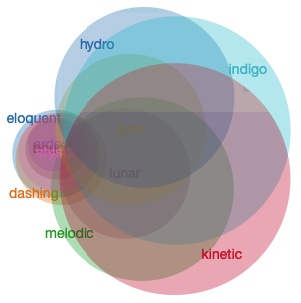
\includegraphics[width=0.4\linewidth]{ros_packages_stat.png}}
					\caption{Диаграмма, показывающая статистику распределения пакетов для различных версий ROS из глобального репозитория ROS Index}
					\label{fig:ROSPackages}
				\end{figure}
			
			\subsection{Концепции ROS}
				Ниже приведён список концепций рассматриваемого фреймворка для понимания описываемой в данном отчёте: 
				\begin{itemize}
					\item {\textbf{Узел} - это процесс, выполняющий вычисления. Каждый узел написание с использованием клиентских библиотек ROS. Используя методы связи, узлы могут общаться друг с другом и обмениваться данными. Для этого создаются узлы-подписчики, и узлы-публикаторы.}
					\item {\textbf{Мастер} - обеспечивает регистрацию и работоспособность запущенных узлов.}
					\item {\textbf{Сообщение} - простая структура данных, содержащая типизированное поле, которое может содержать целый набор данных, отправляемых на другой узел. Помимо стандартных типов сообщений\footnote{Такие как целые, с плавающей точкой, логические, строковые...} возможна отправка заранее обозначенных собственных типов сообщений.}
					\item {\textbf{Топик} - именованная шина данных, используемая узлами для отправки сообщений. Публикующий и подписанный узел не знают о существовании друга друга. Благодаря тому что каждая тема имеет уникальное имя, любой узел может получить доступ к данному топику и отправляет через него данные, при условии соблюдения заранее оговорённых передаваемых типов, данным топиком}
					\item {\textbf{Сервисы} - реализация удалённого вызова процедур\footnote{RPC} в ROS. В некоторых случаях модель связи публикации и подписки может не подходить. В этих случаях и применяют взаимодействия в виде сервисов (схема запрос/ответ), при котором один узел может запросить выполнение процедуры для другого узла, ожидая какого-то обязательного ответа\footnote{В случае использования схемы с подписчиками и публикаторами доставка сообщений и ответ не гарантируются}\cite{bib:ROSDefinition}. }
				\end{itemize}
				
				Схема взаимодействия ROS изображена на Рисунке \ref{fig:ROSScheme} \fxnote{цитата del Corral Tercero, Gonzalo \& Macías, Miquel. (2018). Training a drone using ROS and OpenAI Gym.}.
				
				\begin{figure}[h]
					\center{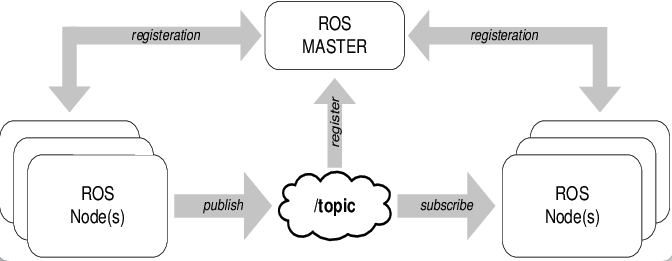
\includegraphics[width=0.8\linewidth]{ros_scheme.png}}
					\caption{Схема взаимодействия ROS}
					\label{fig:ROSScheme}
				\end{figure}
				
		\section{Реализуемые узлы}
			В терминах ROS для решения задачи, поставленной в ВКР необходимо реализовать ряд узлов, которые будут взаимодействовать друг с другом.
			
			\subsection{Узел камеры}
			 	Для поиска объектов, встречающихся на пути следования робота, необходимо озаботиться реализацией одним из "органов чувств" робота - зрением. 
				
				Если на изображении будет обнаружен целевой объект, то роботу необходимо будет его локализовать, подъехать и обозначить его местоположения на карте местности, которая будет строиться исходя из показаний другого сенсора, установленного на роботе (подробнее в разделе \ref{sec:LiDAR}. Визуализация такого обнаружения объектов на изображении показано на Рисунке \ref{fig:ObjectDetectionExample}.
				
				\begin{figure}[h]
					\center{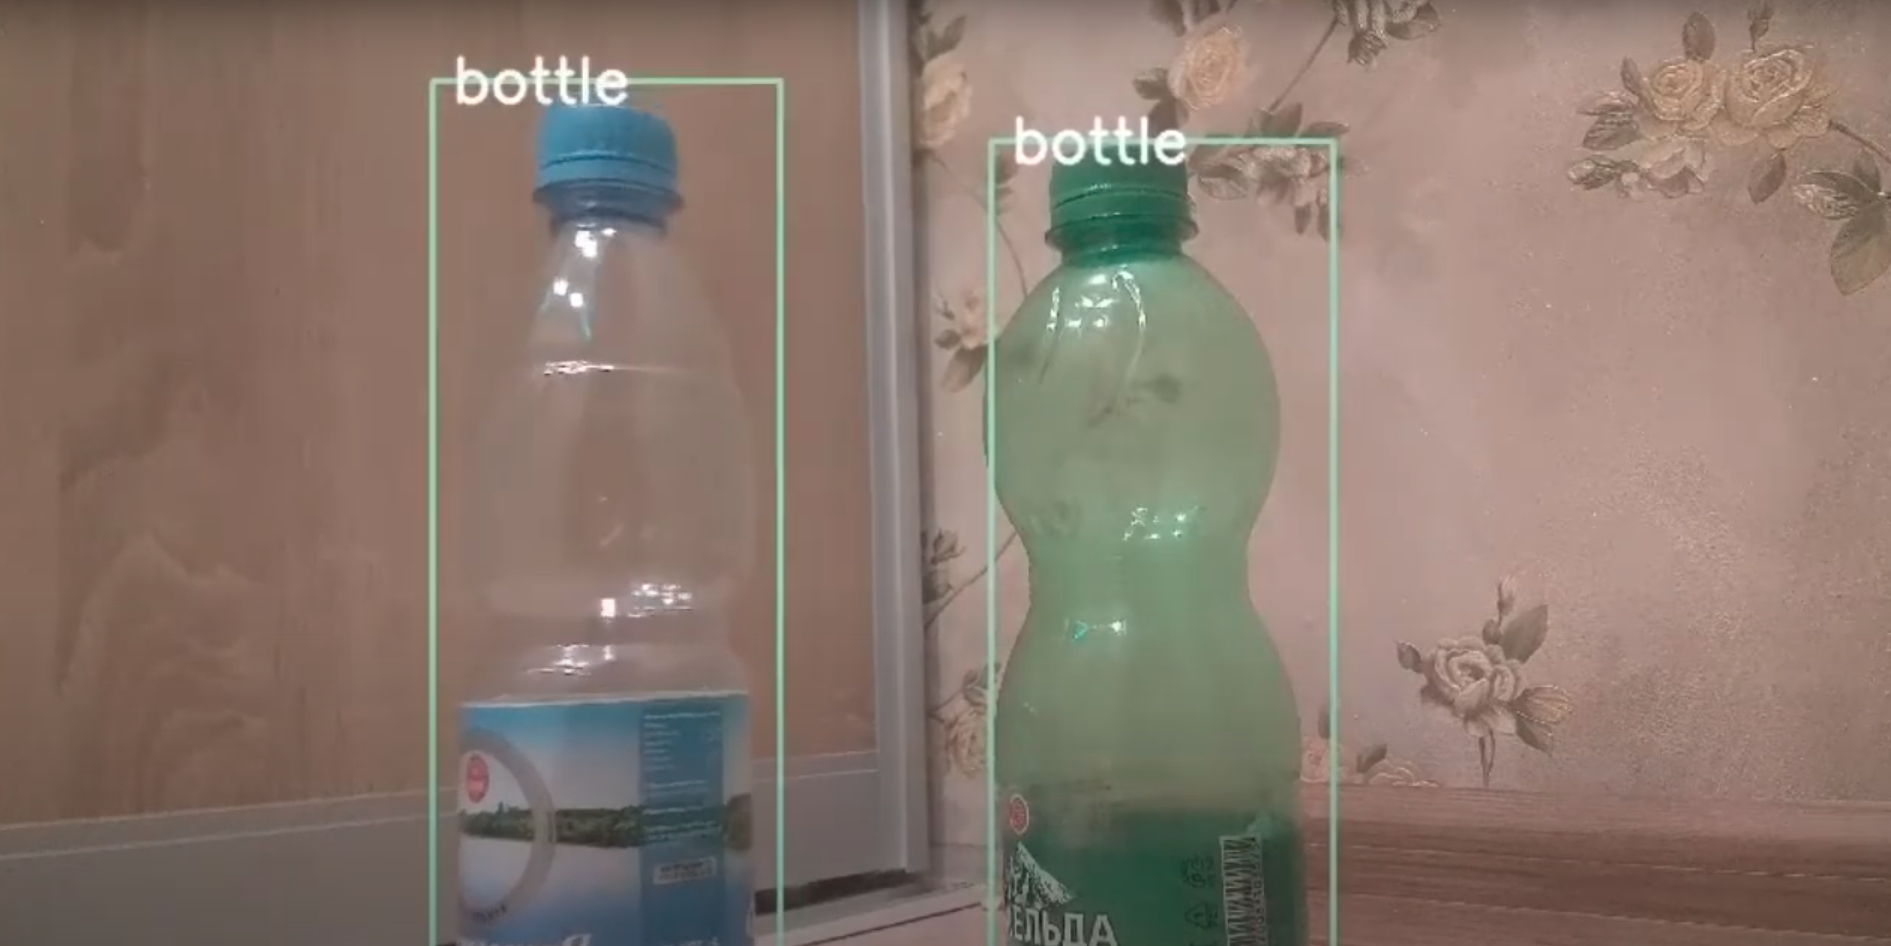
\includegraphics[width=0.6\linewidth]{object_detection_example.png}}
					\caption{Пример распознавания двух целевых объектов роботом}
					\label{fig:ObjectDetectionExample}
				\end{figure}
							 
			 	Компьютер, которым оснащён робот предоставляет высокоскоростной интерфейс CSI\fxnote{цитата тут}, позволяющий читать изображение высокого разрешения с миниатюрной видеокамеры. В качестве видеокамеры выбрана Sony IMX219 с разрешением 3280 x 2464 пикселей и углом обзора 70 градусов, изображённая на Рисунке \ref{fig:csiCam} \fxnote{цитата тут}. 
			 	\begin{figure}[h]
					\center{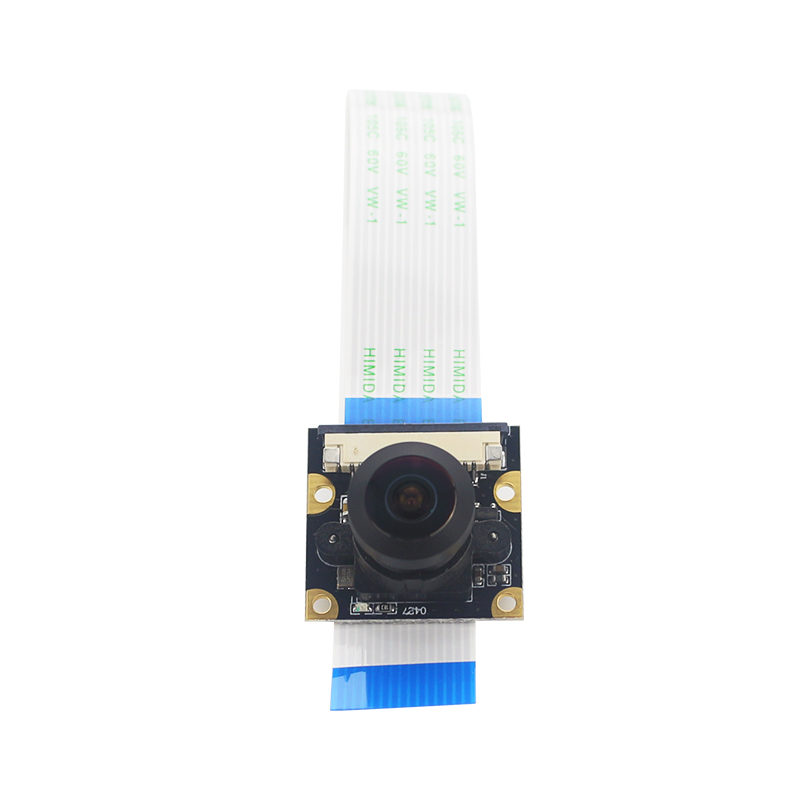
\includegraphics[width=0.4\linewidth]{csi_camera.jpg}}
					\caption{CSI камера для Nvidia Xavier NX}
					\label{fig:csiCam}
				\end{figure}
				
				Задачи данного узла:
				\begin{itemize}
					\item Чтение <<сырого>> изображения с видеокамеры с шины CSI;
					\item Преобразование считанных данных в формат <<sensors\_msgs/Image>>, приведённой в Листинге \ref{lst:ImageMsg} \fxnote{цитата тут http://docs.ros.org/en/noetic/api/sensor\_msgs/html/msg/Image.html};
					\item Публикация в соответствующий ROS топик "/image".
				\end{itemize}
				
				\begin{lstlisting}[language=C,caption={Формат сообщения sensors\_msgs/Image},label={lst:ImageMsg}]
std_msgs/Header header
uint32 height
uint32 width
string encoding
uint8 is_bigendian
uint32 step
uint8[] data
				\end{lstlisting}
				
			\subsection{Узел LIDAR} \label{sec:LiDAR}
				Данный узел будет являться вторым органом зрения робота, обеспечивая его информацией об окружающем пространстве на расстоянии от 10 см до 10 метров. Обеспечивать такое зрение будет лазерный сканер YDLIDAR X4, изображённый на рисунке \ref{fig:ydlidarx4}\cite{bib:ydlidarx4}. Он подключается по серийному порту и способен считывать облако точек с частотой до 12 Гц\cite{bib:ydlidarx4}. 
				
				\begin{figure}[h]
					\center{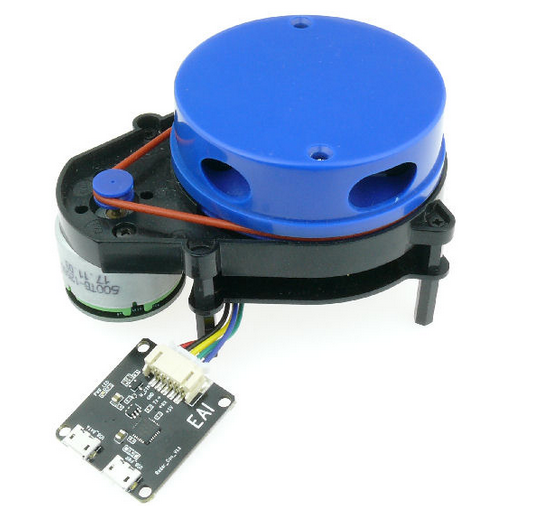
\includegraphics[width=0.4\linewidth]{ydlidar_x4.png}}
					\caption{YDLIDAR X4}
					\label{fig:ydlidarx4}
				\end{figure}
				
				В задачи данного узла входит:
				\begin{itemize}
					\item Чтение <<сырых>> данных об интенсивности отражения лазера от объекта;
					\item Перевод этих данных в формат <<sensor\_msgs/LaserScan>>, приведённой в Листинге \ref{lst:LaserScanMsg} \fxnote{цитата тут http://docs.ros.org/en/noetic/api/sensor\_msgs/html/msg/LaserScan.html};
					\item Публикация в ROS топик "/scan".
				\end{itemize}
				
				\begin{lstlisting}[language=C,caption={Формат сообщения sensor\_msgs/LaserScan},label={lst:LaserScanMsg}]
std_msgs/Header header
float32 angle_min
float32 angle_max
float32 angle_increment
float32 time_increment
float32 scan_time
float32 range_min
float32 range_max
float32[] ranges
float32[] intensities
				\end{lstlisting}	
				
				Результатом работы данного узла является облако точек, которое показывает препятствия вокруг робота\cite{bib:lidarDescription}. Пример визуализации можно увидеть из программы RVIZ на Рисунке \ref{fig:LaserScan} \fxnote{цитата тут http://www.hessmer.org/blog/tag/ros/}.
				
				\begin{figure}[h]
					\center{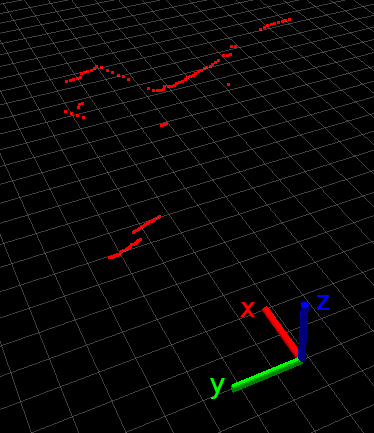
\includegraphics[width=0.4\linewidth]{LaserScan.png}}
					\caption{Пример визуализации облака точек}
					\label{fig:LaserScan}
				\end{figure}
				
			\subsection{Узел движения} \label{sec:Movement}
				Для того чтобы приводить шасси робота, изображённое на Рисунке \ref{fig:Robot} в движение, необходимо контролировать два установленных на него электродвигателя. 
				
				\begin{figure}[h]
					\center{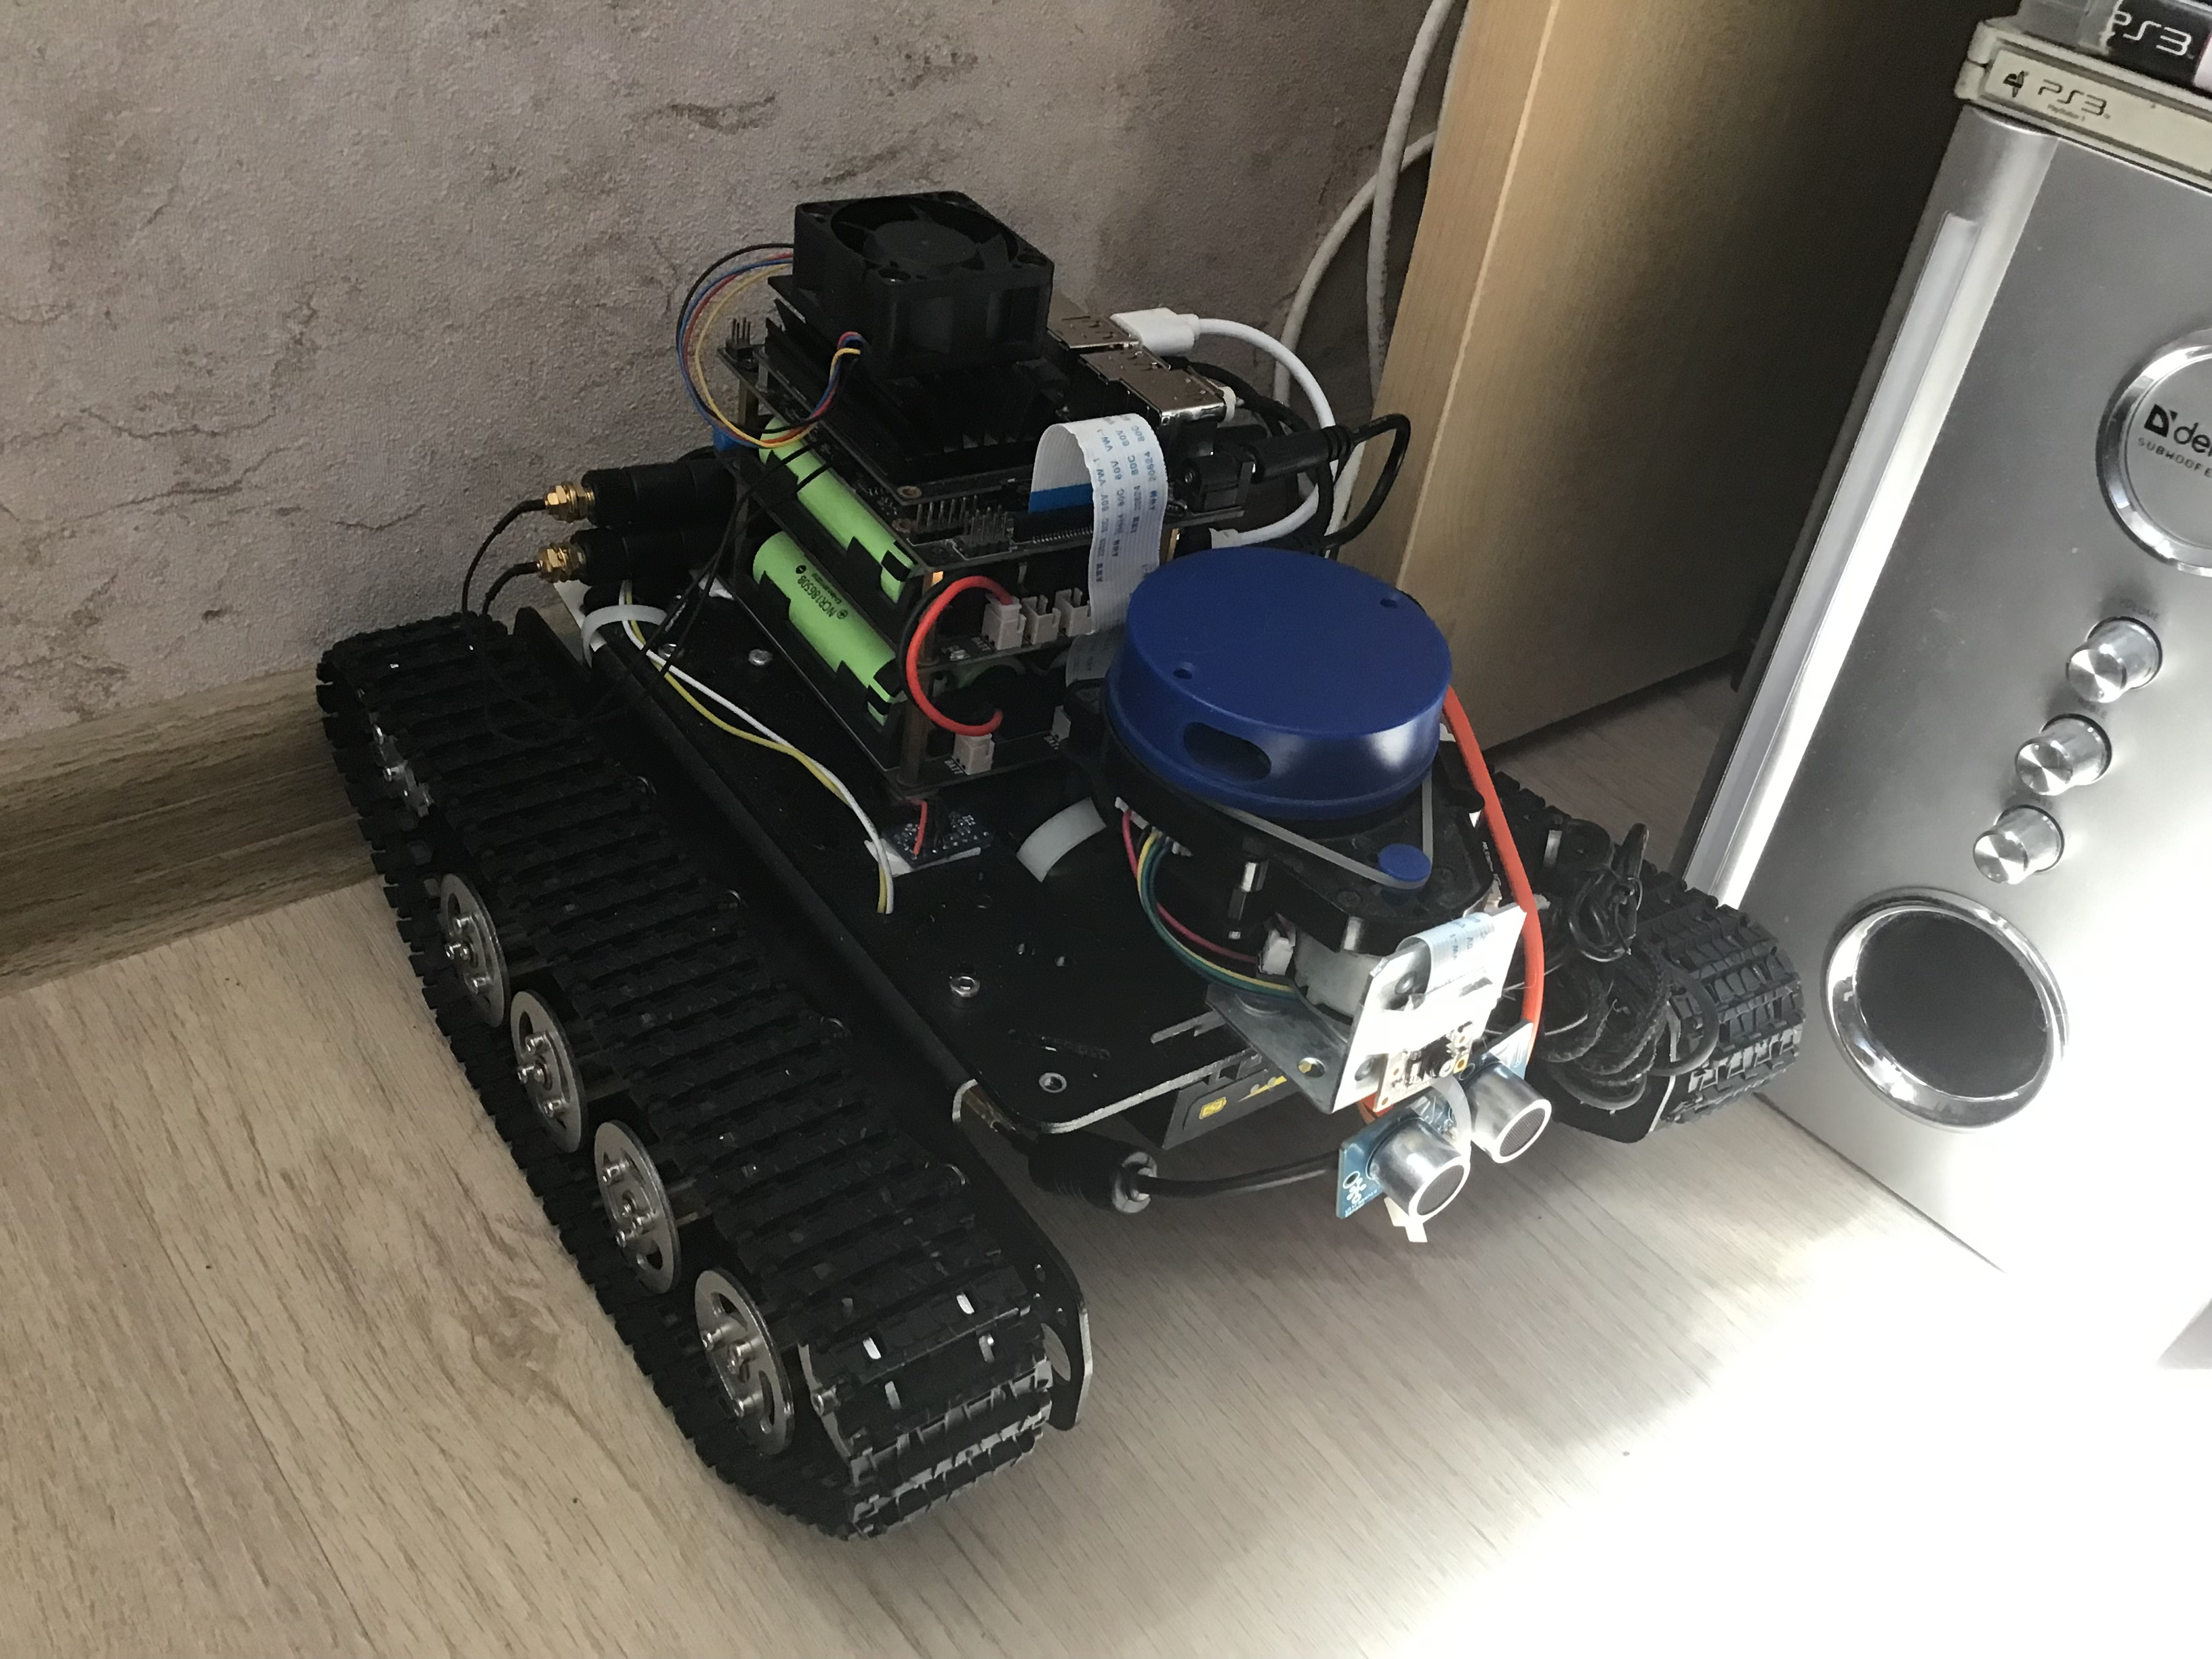
\includegraphics[width=0.6\linewidth]{robot.jpeg}}
					\caption{Шасси робота}
					\label{fig:Robot}
				\end{figure}
				
				С этой задачей необходимо правильно работать как с аппаратной, так и с программной стороны. Для этого необходимо:
				
				\begin{itemize}
					\item Одновременно управлять силой тока двух электродвигателей;
					\item Определять расстояние и направление, пройденное каждой гусеницей;
					\item Без задержек взаимодействовать с остальными участниками сети ROS.
				\end{itemize}
				
				\subsubsection{Аппаратное управление двигателями}
					Для того чтобы обеспечить неукоснительное команд от управляющего узла ROS в виде показанного на Листинге \ref{lst:TwistMsg}\fxnote{цитату прикрепить http://docs.ros.org/en/noetic/api/geometry\_msgs/html/msg/Twist.html} формата сообщения <<geometry\_msgs/Twist>> и соблюдать заданную скорость и направление движения, необходимо уметь регулировать уровень электрического входного напряжения на каждом двигателе по отдельности при помощи ШИМ-модуляции\footnote{Широтно-импульсная модуляция (ШИМ) - метод используемый для регулирования эффективного напряжения, подаваемого на двигатель, с целью изменения скорости вращения. Изменение подаваемого на двигатель напряжения с помощью потенциометра неэффективно, посколько сопротивление двигателя намного меньше, чем сопротивление потенциометра, в результате чего последний использует всю мощность источника напряжения.}, схематично изображённой на Рисунке \ref{fig:Shim}\fxnote{цитата https://clck.ru/h3Ndo}. При этом устройство, выполняющее данную задачу должно быть интерфейсно совместимо с управляющим компьютером. 
					
					\begin{lstlisting}[language=C,caption={Формат сообщения geometry\_msgs/Twist},label={lst:TwistMsg}]
geometry_msgs/Vector3 linear
geometry_msgs/Vector3 angular
					\end{lstlisting}	
					
					\begin{figure}[h]
						\center{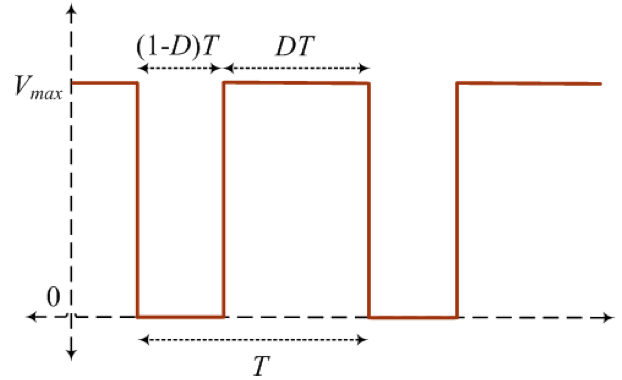
\includegraphics[width=0.6\linewidth]{shim.png}}
						\caption{Импульсный сигнал}
						\label{fig:Shim}
					\end{figure}
					
					В качестве такого устройства было выбран двухканальный драйвер двигателя Grove Motor Driver, изображённый на Рисунке \ref{fig:GroveMotorDriver}. В его сердце лежит управляющий чип L298 и он может управлять двигателями с уровнем напряжения от 2.5В до 13.5В\fxnote{цитата https://www.seeedstudio.com/Grove-I2C-Motor-Driver-with-L298.html}. Интерфейс управления - I2C, совместимый с управляющим компьютером робота.
					
					\begin{figure}[h]
						\center{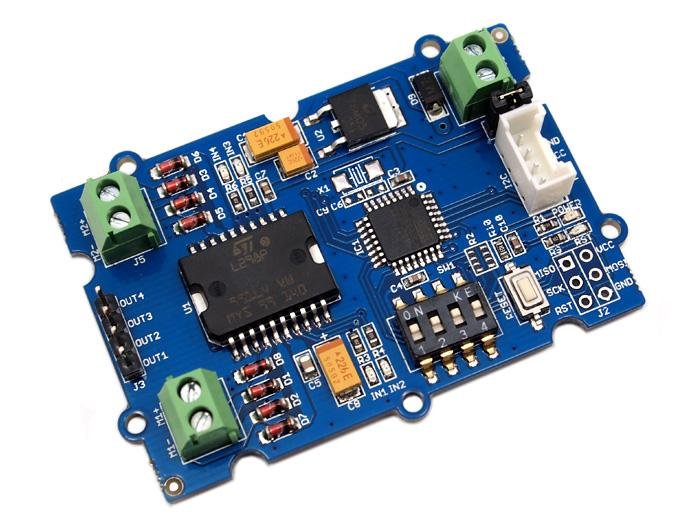
\includegraphics[width=0.6\linewidth]{GroveMotorDriver.jpg}}
						\caption{Драйвер двигателя Grove Motor Driver}
						\label{fig:GroveMotorDriver}
					\end{figure}
					
				\subsubsection{Одометрия}
					Далее определение расстояния и направления, пройденного каждой гусеницей будет называться одометрией. Для решения данной задачи необходимо получать информацию о фактических оборотах электродвигателей робота, так как по каким-либо физическим причинам она может отличаться от ожидаемой.
					
					Для подсчёта фактических оборотов будут использоваться датчики Холла, встроенные в электродвигатель робота, изображённый на Рисунке \fxnote{рисунок тут}.
					
					Датчики Холла выдают электрический импульс (в нашем случае 3.3В) при прохождении колесом двигателя определённой точки\fxnote{цитата книги https://booksee.org/book/349379}. Осцилограмму датчика Холла можно увидеть на Рисунке \fxnote{рисунок}. 
					
					С программной стороны в реальном времени мы должны подсчитывать данные импульсы и на основе очерёдности сигналов с двух датчиков Холла, установленных на оба электродвигателя делать вывод о направлении движения, а также публиковать сообщение одометрии в стандартном формате сообщений ROS <<nav\_msgs/Odometry>>, описанном в Листинге \fxnote{листинг и цитата тут}. Заниматься этой работой будет микрокомпьютер Teensy 4.0, изображённый на Рисунке \fxnote{рисунок} \fxnote{цитата}.
					
			\subsection{Узел SLAM} \label{sec:Movement}
				Программным сердцем данной работы является узел SLAM\footnote{Simultaneous Localisation and Mapping}, реализуемый открытой программной реализацией Google Cartographer. SLAM (одновременная локализация и картографирование) — это метод, используемый для автономных транспортных средств, который позволяет одновременно создавать карту и локализовать себя на этой карте. Алгоритмы SLAM позволяют картографировать неизвестные среды и обычно это используется для выполнения таких задач, как планирование пути и обход препятствий.
				
				Для определения препятствий будет использоваться облако точек, приходящее от LiDAR. На основе получаемого облака и текущего местоположения робота, которое высчитывается исходя из данных одометрии, мы будем строить карту местности, изображённую на Рисунке \fxnote{рисунок тут}. 
				
				Эта карта позволит роботу самостоятельно прокладывать маршрут до следующей планируемой точки. Выбор планируемой точки осуществляется следующим образом:
				
				\begin{enumerate}
					\item Если в кадре есть целевой объект и ранее он не был обозначен на карте, мы стремимся к нему;
					\item Если мы находимся достаточно близко к целевому объекту, помечаем его на карте и выбираем следующую точку;
					\item Во всех остальных случаях мы выбираем следующую случайную точку близкой к неисследованной области с возможным безпрепятственным проездом туда. 
				\end{enumerate}
					
			\section*{Заключение}
				Таким образом был разработан и описан мобильный автономный робот, изображённый на Рисунке\fxnote{рисунок тут} с функцией поиска целевых объектов на карте, который может быть применён в задачах по исследованию опасных объектов, разведке и сборе данных. Безусловно, данная модель для применения в реальных задачах требует значительных доработок в плане точности движения и локализации, и не является идеальной.
					
						
		\section*{Вступление}
			В ходе практики я работал над корректным подсчётом пройденного роботом расстоянием. Это позволит роботу самому оценивать его текущее местоположение на карте, выстраиваемой при помощи лазерного сканера LiDAR. Сам робот представляет собой платформу на двух гусеницах и оснащён двумя электродвигателями, драйвером, лазерным сканером и компьютером, управляющий процессом движения. Он изображён на Рисунке \ref{fig:Robot}.
			
			\begin{figure}[h]
				\center{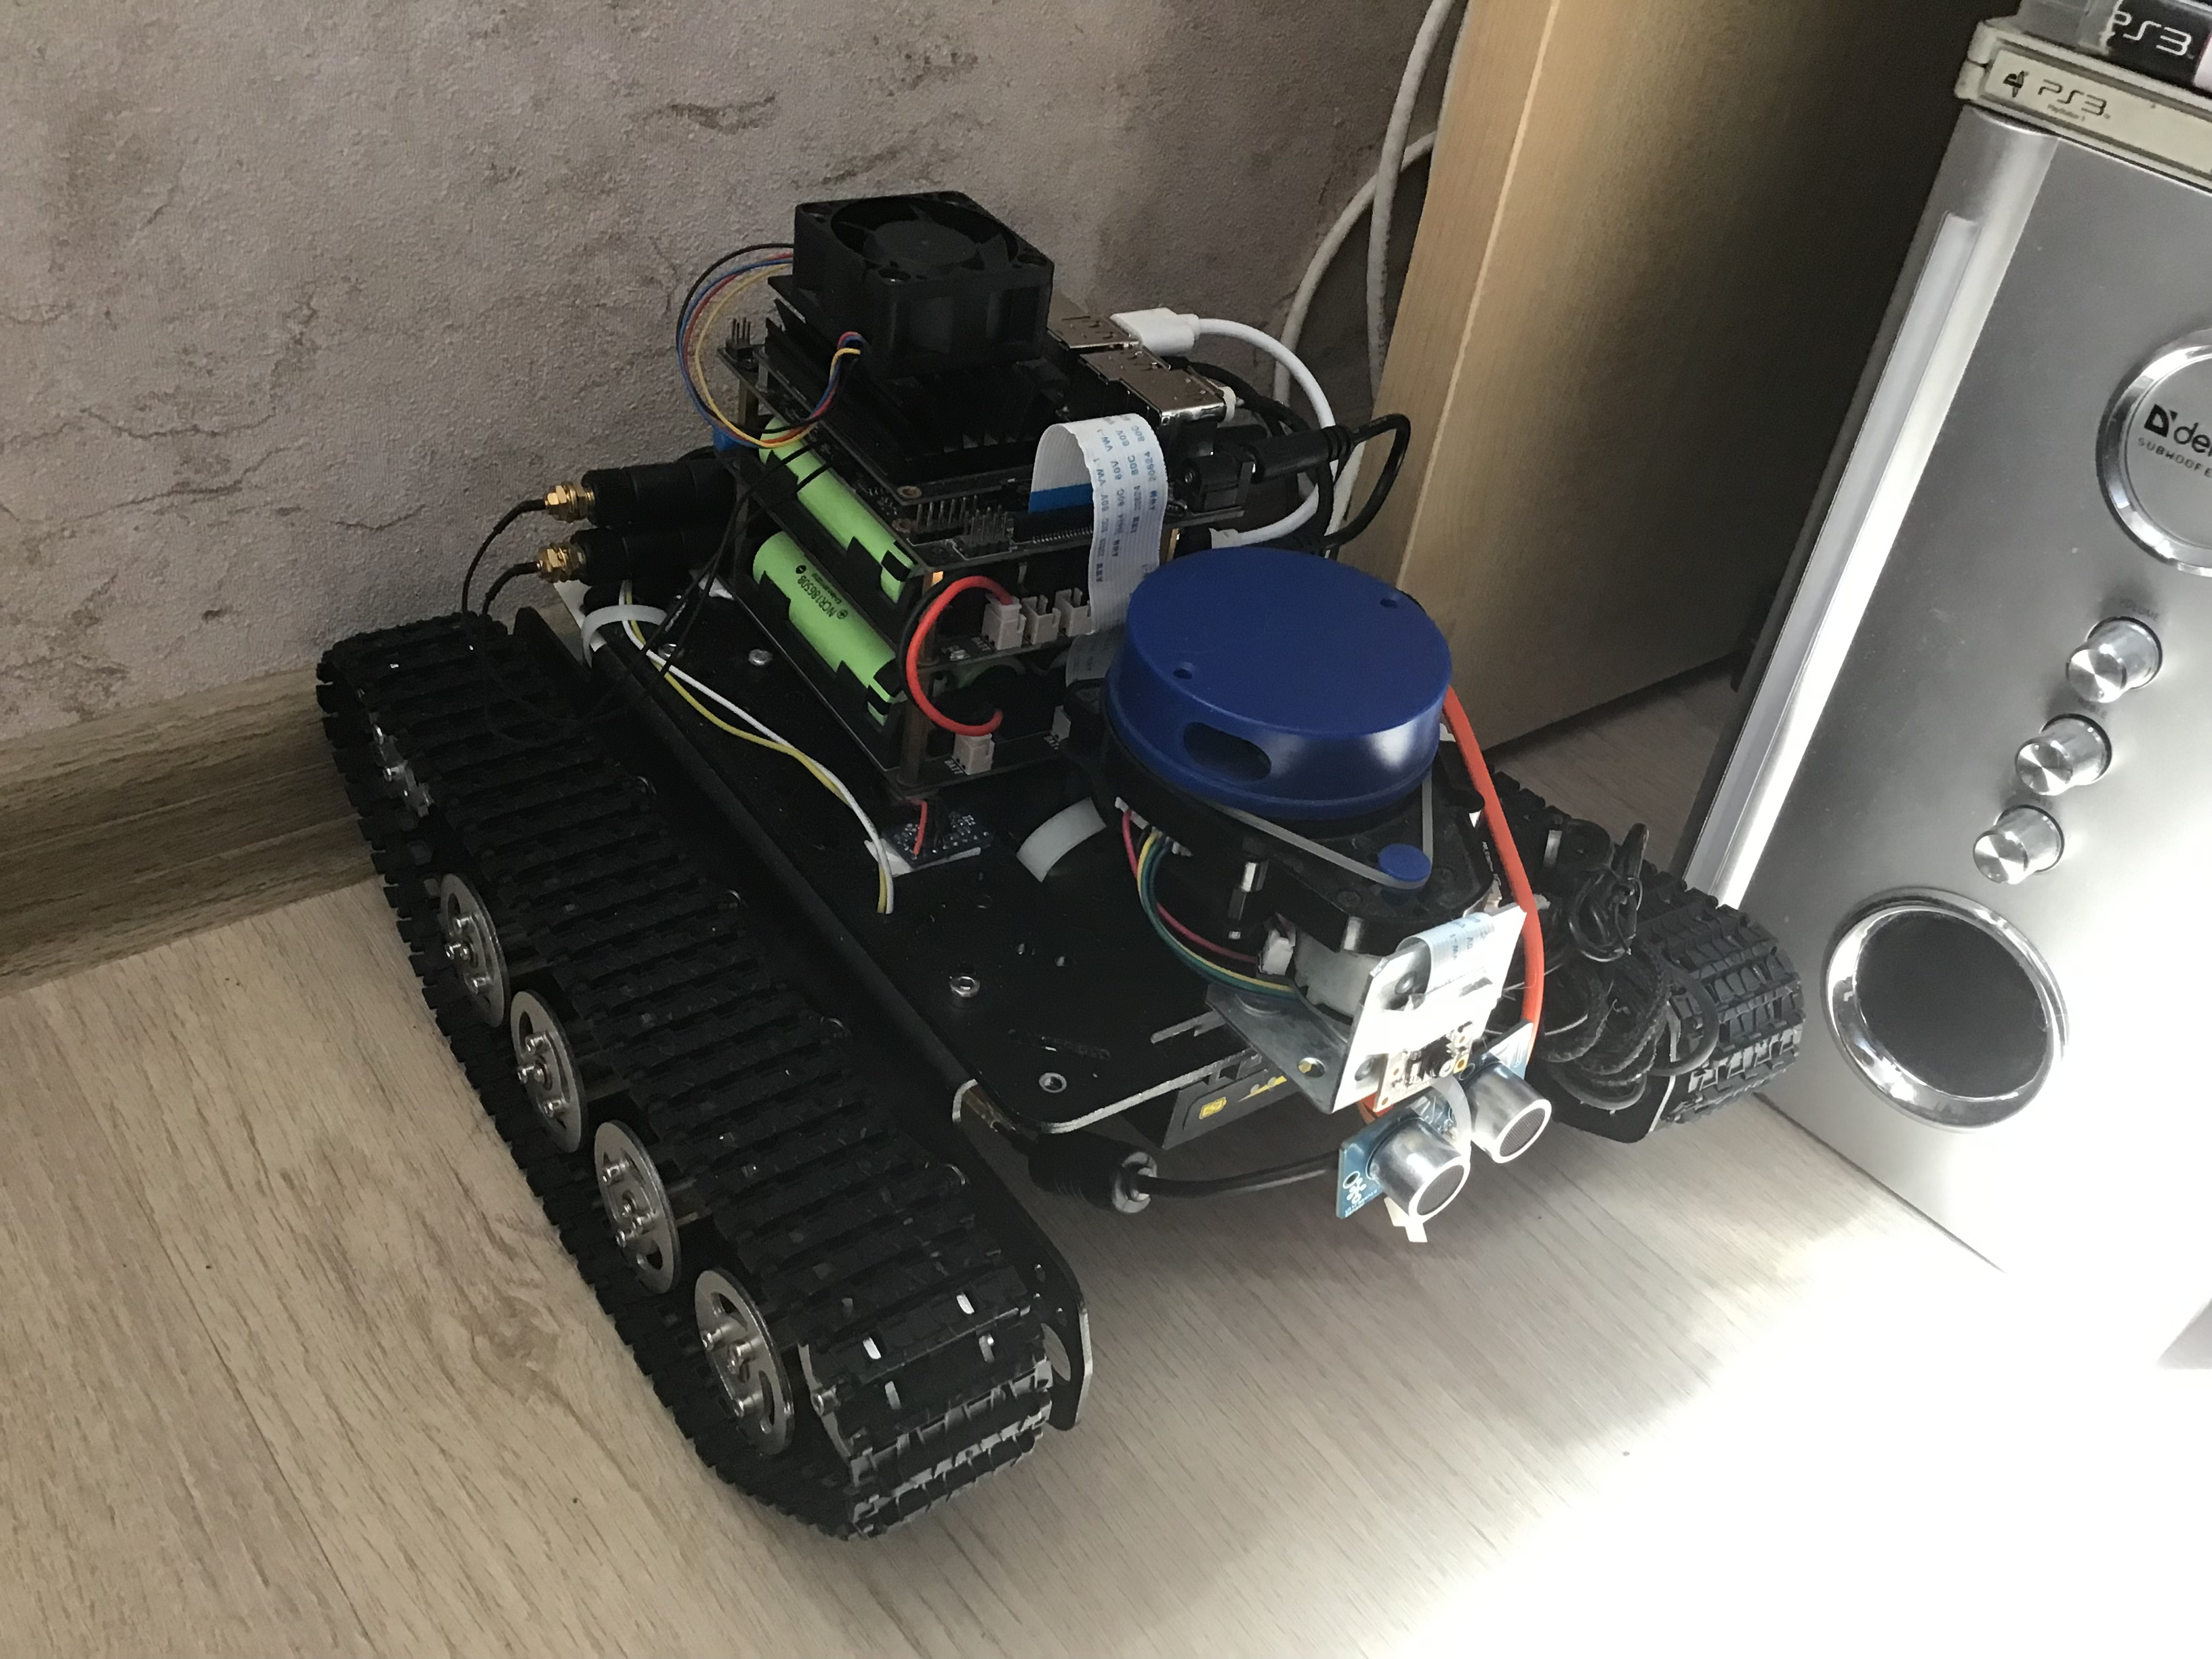
\includegraphics[width=0.6\linewidth]{robot.jpeg}}
				\caption{Робот}
				\label{fig:Robot}
			\end{figure}
			
			Моей задачей стало исправление некорректного подсчёта числа оборотов колеса производимых на ведущей части гусеницы робота. Для успешного построения карты местности (пример изображён на Рисунке \ref{fig:Map}) при помощи лазерного сканера, изображённого на Рисунке \ref{fig:X4} роботу необходимо решать задачу локализации в пространстве. Погрешностей в определении местоположения должно быть как можно меньше, они напрямую будут влиять на выстраиваемую карту местности. Будут возникать смещения или ещё хуже - артефакты\footnote{объекты на карте, которых в реальности не существует}.
			
			\begin{figure}[h]
				\center{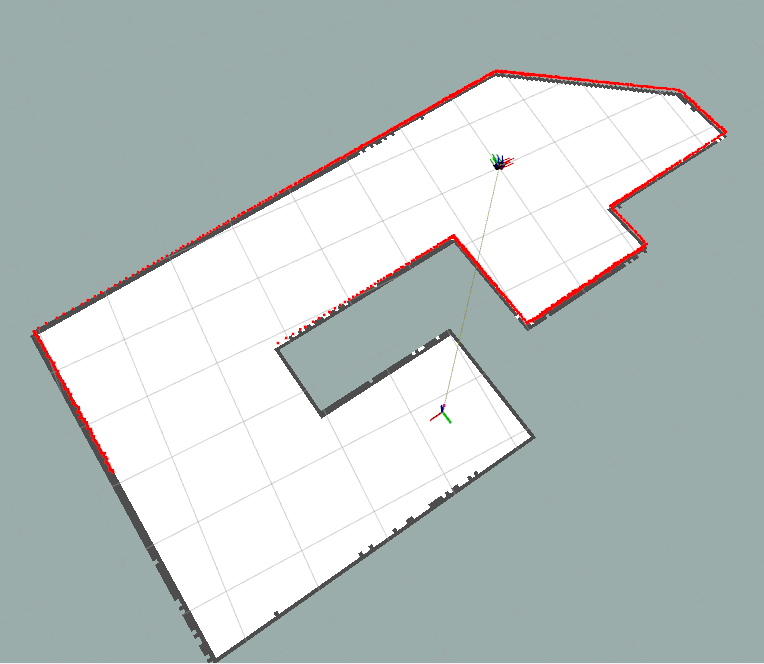
\includegraphics[width=0.6\linewidth]{rviz_map.png}}
				\caption{Карта местности, построенная при помощи лазерного сканирования}
				\label{fig:Map}
			\end{figure}
			
			\begin{figure}[h]
				\center{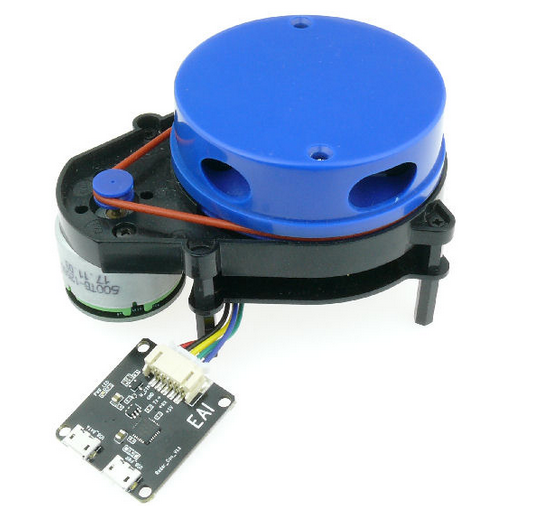
\includegraphics[width=0.6\linewidth]{ydlidar_x4.png}}
				\caption{Лазерный сканер YDLIDAR X4}
				\label{fig:X4}
			\end{figure}
			
			На данном роботе возможно реализовать три способа локализации в пространстве:
			\begin{enumerate}
				\item Анализ смещения облака точек;
				\item Подсчёт одометрии;
				\item Первые два способа вместе, корректирующие показатели друг друга.
			\end{enumerate}
			
			Такие способы локализации, как триангуляция на основе заранее установленных радиомаяков и спутниковая связь Глонасс не рассматриваются ввиду требования полной автономности робота.
			
		\section*{Практика}
			Моей задачей является - "исправление расчета оборотов ведущего колеса гусеничного шасси робота". На основе этих оборотов считается фактически пройденное роботом расстояние после применения команды движения в определённую сторону. Обнаружилось, что получаемые значения оборотов отличались от ожидаемых при высокой загруженности управляющего компьютера. Изначально исправлению подлежала только программная часть робота, однако в ходе работы выяснилось, что природа ошибки кроется в операционной системе робота. 
			
			Принцип получения показателей пройденного роботом расстояния следующий:
			\begin{itemize}
				\item Робот включается и инициализирует среду ROS\footnote{Robot Operating System};
				\item Включается система навигации робота, которая требует лазерный сканер и текущее расстояние, пройденное гусеницами;
				\item Запускается лазерный сканер и происходит инициализация аппаратного интерфейса GPIO с цифровыми электрическими входами;
				\item Навигационная система по шине I$^2$C даёт команду драйверам двигателя на движение;
				\item Датчики Холла, установленные на двигателях робота подают электрический сигнал 3.3 вольт в момент прохождения колесом одного оборота.
				\item Аппаратный интерфейс GPIO считывает данный сигнал и суммирует все такие обороты;
				\item На основе новых пройденных роботов подсчитывается пройденное роботом расстояние.
			\end{itemize}
			
		\section*{1 этап}
			Первоначально я посчитал, что причиной расхождения показателей является подвисание программы на каком-либо из циклов в программном коде и при высокой загруженности мы просто не успеваем исполнить код, отвечающей за чтение цифрового сигнала на интерфейсе GPIO. В таком случае вполне возможно мы могли недосчитаться каких-то оборотов колеса и избавление от таких циклов станет решением проблемы.
			
			Т.к. речь идёт о программном коде робота и мы имеем дело с Robot Operating System, оперирующей с входными данными, как с входящими в неё топиками, которые публикуют другие узлы, я нашёл какой узел отвечает за публикацию и суммирование текущих оборотов двигателя. Искать долго не пришлось, но никаких бесконечных циклов в коде узла и библиотеки Jetson.GPIO, которую он использует найдено не было. Каких-либо мест в коде, где исполнение узла могло бы застревать найдено не было. 
			
			Мною была выдвинута идея о том, что такие просчёты со стороны узла напрямую связаны с природой операционной системы Ubuntu, используемой на роботе. Данная ОС не является системой, нацеленной на исполнение команд в режиме реального времени, а это значит, что в момент прохождения ведущим колесом робота датчика Холла мы не можем гарантировать квант времени от операционной системы на исполнение программы нашего узла, а значит не можем и гарантировать подсчёт всех оборотов колеса. Примерная схема такого просчёта представлена на Рисунке \ref{fig:Miscount}
			
			\begin{figure}[h]
				\center{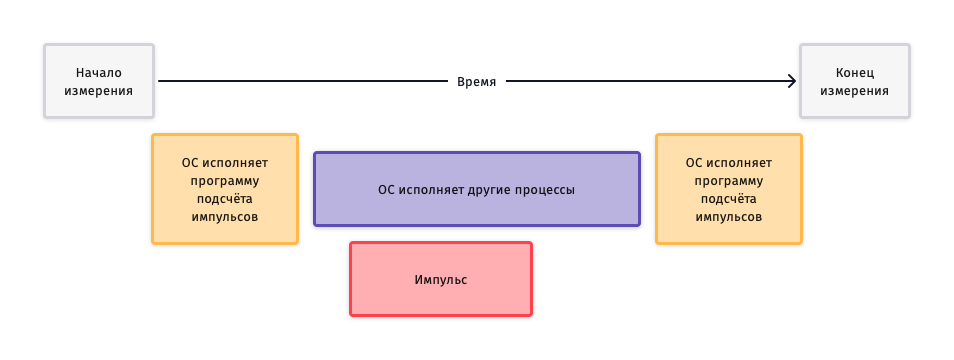
\includegraphics[width=\linewidth]{Miscount.png}}
				\caption{Пример импульса, который не будет подсчитан программой}
				\label{fig:Miscount}
			\end{figure}
			
			Заручившись поддержкой тематических интернет-форумов и своего научного руководителя, я приступил ко второму этапу...
			
		\section*{2 этап}
			Выходом из данной ситуации стало бы использование операционной системы реального времени, такой как QNX\footnote{QNX (произносится «кьюникс», «кью-эн-экс») — POSIX-совместимая операционная система реального времени, предназначенная преимущественно для встраиваемых систем. Считается одной из лучших реализаций концепции микроядерных операционных систем.}, но это стало не позволительной роскошью для данного робота в следствии отсутствия какой-либо рабочей реализации используемого фреймворка ROS для данной ОС, а также высокая стоимость лицензии.
			
			По названным выше причинам было решено некоторый микроконтроллер, который удовлетворял следующим требованиям:
			\begin{enumerate}
				\item Принимает электрические сигналы в реальном времени без просчётов
				\item Способна коммуницировать с Robot Operating System
				\item Является компактным и энергоэффективным решением
			\end{enumerate}
			
			Под эти требования отлично подошёл микроконтроллер Teensy 4.0 на базе 32 битного ARM процессора NXP MIMXRT1062DVL6A. Схематичное описание и внешний вид микрокомпьютера представлены на Рисунке 
			
			\begin{figure}[h]
				\center{
					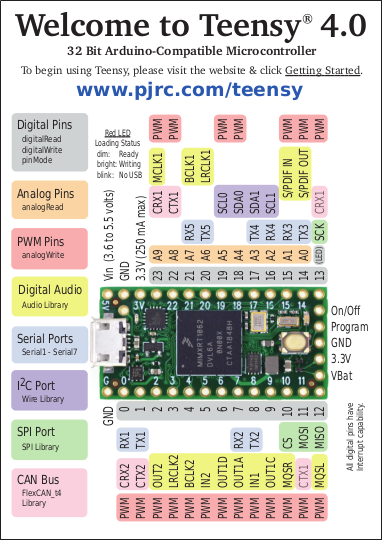
\includegraphics[width=0.45\linewidth]{teensy40_card10a_rev2.png}
					\hspace{0.5cm}
					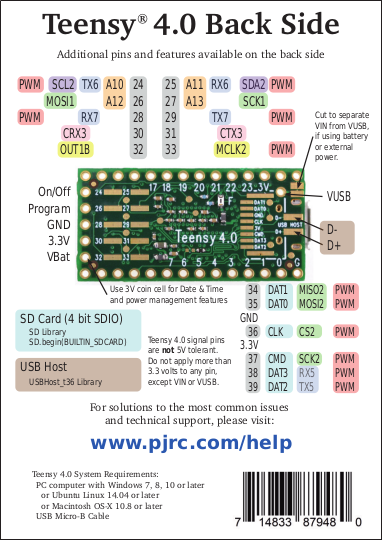
\includegraphics[width=0.45\linewidth]{teensy40_card10b_rev2.png}
				}
				\caption{Описание микрокомпьютера Teensy 4.0}
				\label{fig:TeensyDesc}
			\end{figure}
			
			К нему были подсоединены датчики холла и внешние электропитание 5 вольт. В последствии планируется делегировать на данный микроконтроллер нагрузку, связанную с управлением драйвером электродвигателей робота.
			
			После проверки цепей питания и удостоверившись в корректном прохождении сигналов к микроконтроллеру, я начал реализовывать программную часть.
			
		\section*{3 этап}
			Для реализации программной части необходимо использовать систему разработки Arduino IDE с установленным дополнением TeensyDuino. Это позволяет использовать все библиотеки, доступные для Arduino доступными и для микроконтроллера Teensy 4.0. 
			
			Для коммуникации между основным компьютером NVIDIA Jetson Xavier NX и Teensy 4.0 было решено использовать предоставляемый фреймворком ROS инструмент rosserial. Данный инструмент позволяет при помощи Arduino-совместимой библиотеки и подключения по серийному порту наладить полноценную в рамках ROS коммуникацию в режиме реального времени без необходимости вручную описывать взаимодействие между двумя компьютерами.
			
			Идея взаимодействия будет следующая:
			\begin{enumerate}
				\item На основном компьютере запускается ROS, который при помощи rosserial устанавливает соединение с Teensy
				\item Микроконтроллер считает количество пришедших электрических сигналов
				\item Каждый ROS цикл публикуется количество подсчитанных сигналов
				\item Узел на стороне главного компьютера принимает и обрабатывает данные числа для подсчёта местоположения робота
			\end{enumerate}
			
			Реализация скетча представлена в Листинге ...
			
			\begin{lstlisting}[language=C,caption={Формат сообщения nav\_msgs/Odometry},label={lst:OdometryMsg}]
std_msgs/Header header
string child_frame_id
geometry_msgs/PoseWithCovariance pose
geometry_msgs/TwistWithCovariance twist
			\end{lstlisting}	
			
			После завершения работы мои проверки не показали расхождений в значении подсчитанных оборотов ведущих колёс робота и я посчитал данную задачу завершённой.
			
	\begin{thebibliography}{9}
		\bibitem{bib:FrameworkDefinition} FructCode. Фреймворк - важный инструмент программиста. Обзор HTML/CSS, PHP и Python-фреймворков. - URL:
 \url{https://fructcode.com/ru/blog/features-of-popular-frameworks-html-css-php-and-python-frameworks/} (дата обращения: 16.03.2020). - Текст: электронный.
		\bibitem{bib:ROSDefinition} Lentin Joseph. Mastering ROS for Robotics Programming: Second Edition / Lentin Joseph, Jonathan Cacace. - Birmingham - Mumbai: Packt Publishing Ltd, 2018. - 552 с. - Текст: непосредственный. - с. 7, 20.
		\bibitem{bib:ydlidarx4} Hefei Fidurobot Store. Лазерный Радар-сканер EAI YDLIDAR X4 LIDAR модуль датчика диапазона 10 метров 5 кГц Диапазон частоты EAI YDLIDAR-X4 для ROS. / AliExpress - URL: \url{https://aliexpress.ru/item/32908156152.html} (дата обращения: 16.03.2020). - Текст: электронный.
		\bibitem{bib:lidarDescription} Lentin Joseph. Mastering ROS for Robotics Programming / Birmingham - Mumbai: Packt Publishing Ltd, 2015. - 451 с. - Текст: непосредственный. - с. 270
	\end{thebibliography}
			
	\end{document}